%====================================================================================================
\chapter{Neural networks}

%====================================================================================================
\section{Neural cell}

%----------------------------------------------------------------------------------------------------
\subsection{Neural networks as biological information processing systems}
\FloatBarrier
The basic conducting element in the nervous system is the nerve cell, or neuron.
A neuron has a cell body, dendrite, and axon. The cell body contains many of the organelles 
vital to maintain the cells structure and function, including the nucleus and and is considered the
tropic center of the nerve cell.
The dendrites extend from the cell body and increase the receptive surface of the neuron.
The axon leaves the cell body and connects to other cells. Axons are covered by a lipoproteinaceous
membrane called myelin that insulates the axons from the fluids in the central nervous system.
The site of contact between the axon of one nerve cell and the dendrites and cell body of another 
neuron is the synapse. The cells in the nervous system are classified based on their shapes:
unipolar, bipolar, and multipolar. 
\begin{figure}[htb] 
	\label{fig:neurons}
	\centering
	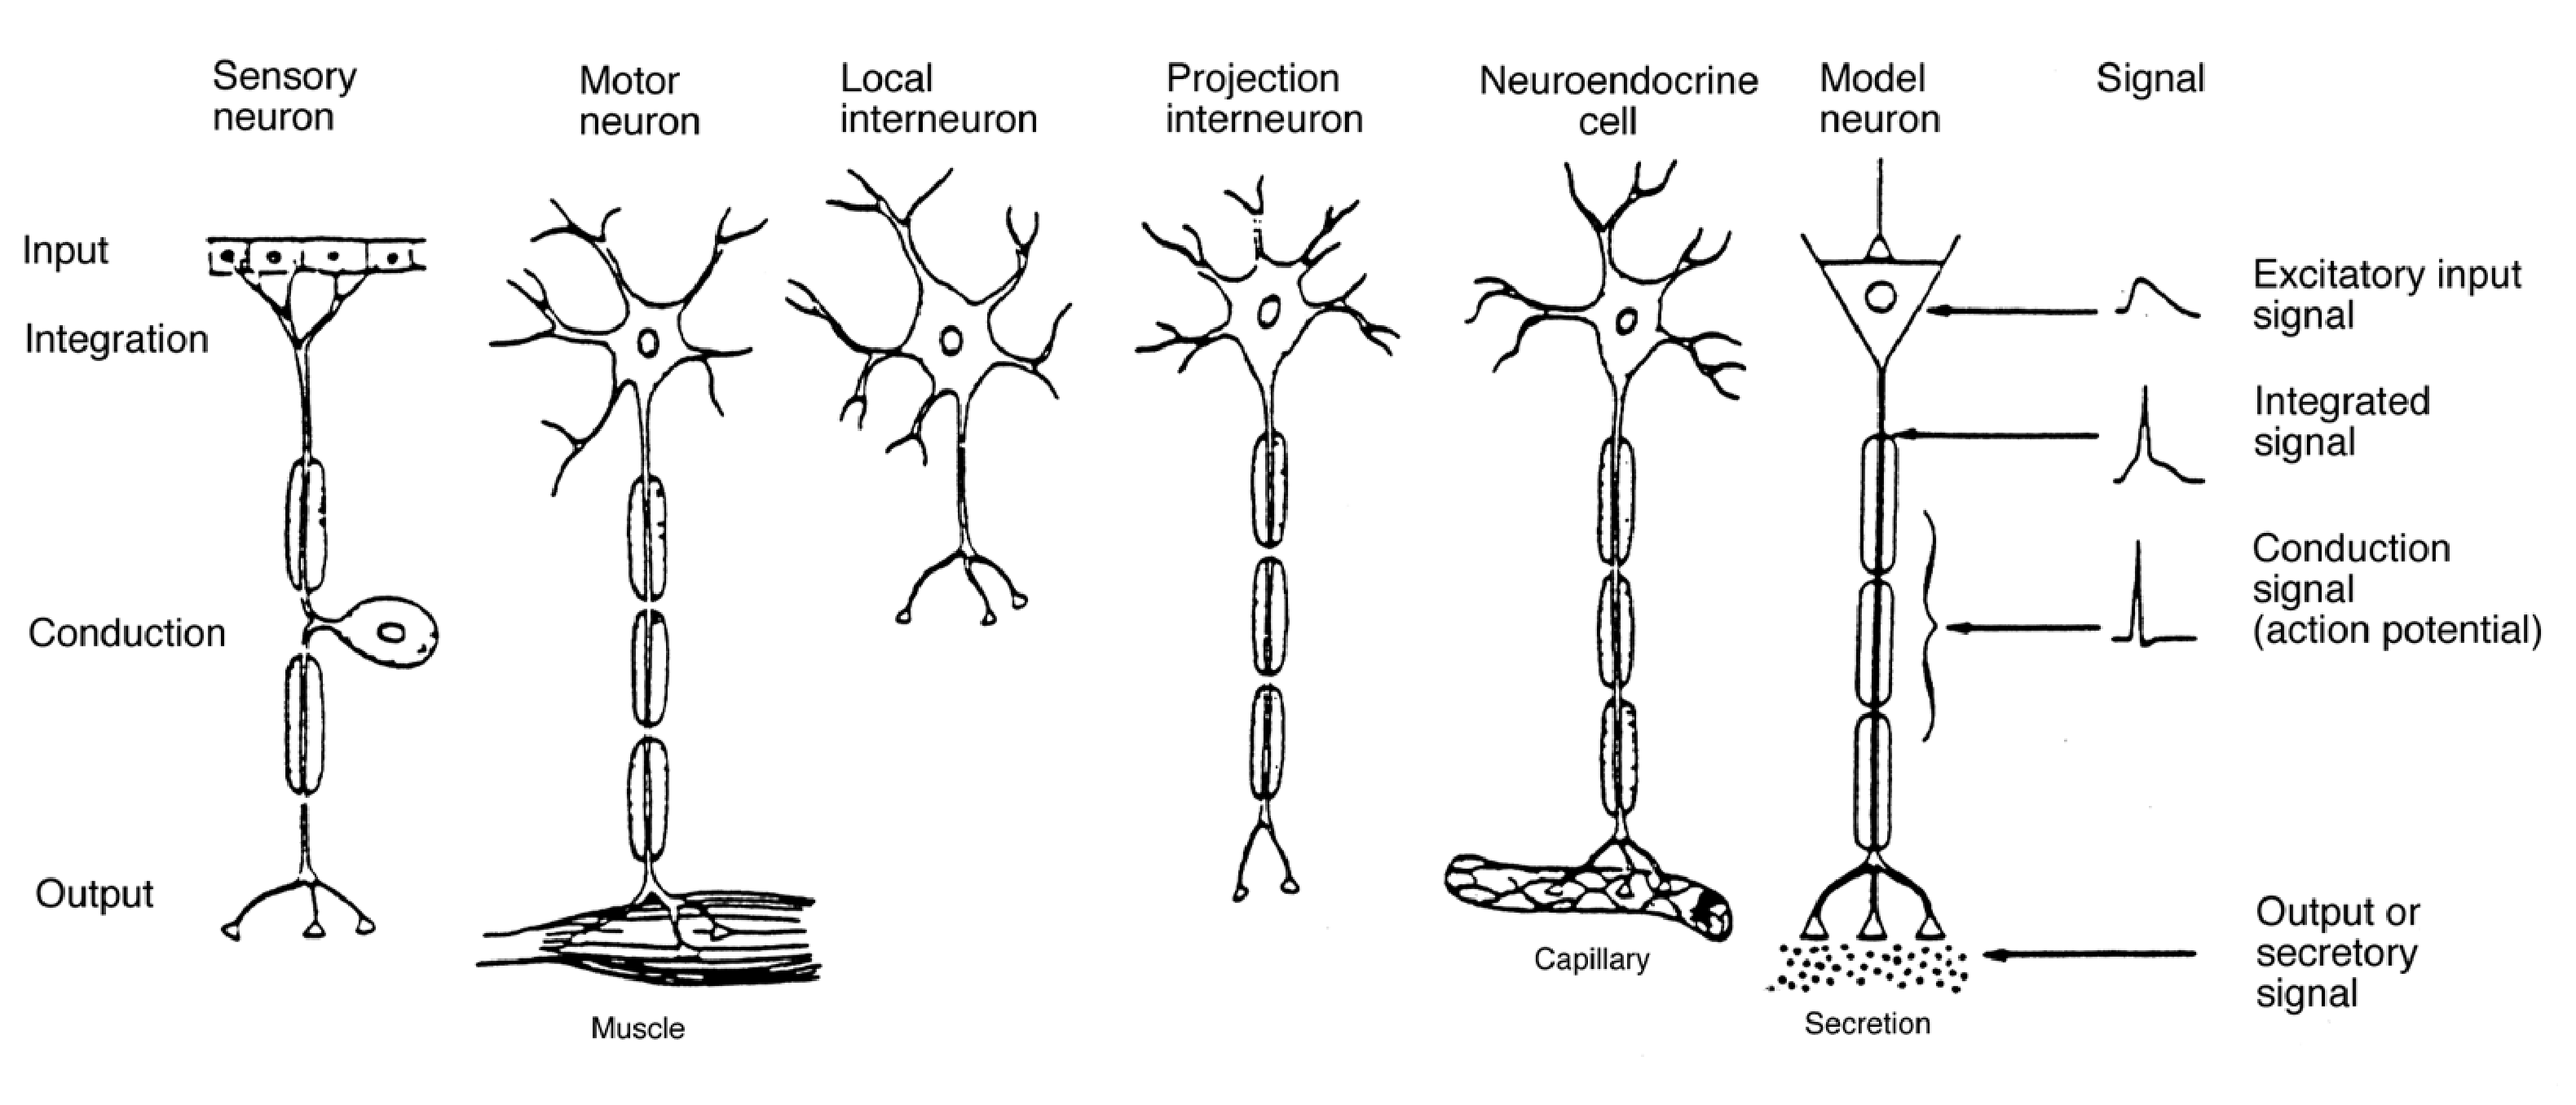
\includegraphics[width=\textwidth]{figures/bio_neurons}
	\caption{Examples of biological neurons}
\end{figure}
In the central nervous system, the nerve cells are supported by glia and blood vessels;
in the peripheral nervous system, they are supported by satellite cells, fibroblasts,
Schwann cells, and blood vessels.
There are three basic categories of neurons:
\begin{itemize}
	\item receptors : the ganglia of the spinal dorsal roots and of the cranial nerves
		with general sensory components,
	\item effectors : the ventral horn cells, motor cranial nerve nuclei, and motor division of
		the autonomic nervous system
	\item Interneurons, the vast majority of the neurons in the central nervous system.
\end{itemize}
The areas in the central nervous system that contain high numbers of neuronal cell bodies are
called gray matter, while the regions that contain primarily myelinated axons are called
white matter. Neurons are organized into ganglia, nuclei, or layered cortices.

There are two basic types of synapses, electrical and chemical, and they differ in location and 
appearance. Electrical synapses are connected by membrane bridges, gap junction and connections,
which permit the electric impulse to pass directly from one cell to the other.
Electric synapses have almost no delay and little chance of misfiring. These synapses are seen in 
many fish.Chemical synapses have a presynaptic side containing vesicles and a gap,
and a postsynaptic side with membrane receptors.
The neurotransmitter released by the action potential is exocytosed and diffuses across the 
synaptic cleft and binds to the specific receptor on the postsynaptic membrane.
Most of the synapses seen in the mammalian central nervous system are chemical.

If the voltage changes by a large enough amount over a short interval, 
the neuron generates an all-or-nothing electrochemical pulse called an action potential. 
This potential travels rapidly along the axon, and activates synaptic connections as it 
reaches them. Synaptic signals may be excitatory or inhibitory, 
increasing or reducing the net voltage that reaches the soma.
\begin{figure}[htb] 
	\label{fig:bio_activation}
	\centering
	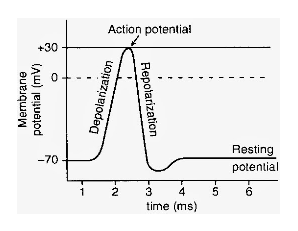
\includegraphics[width=0.6\textwidth]{figures/bio_activation}
	\caption{Examples of biological neurons}
\end{figure}
Chemical synapses consist of presynaptic axon terminals harboring synaptic vesicles and a
postsynaptic region (usually on dendrites) containing neurotransmitter receptors.
These neurotransmitters are made by the presynaptic neuron and stored in synaptic vesicles at
presynaptic terminals.
Whether a synapse is excitatory or inhibitory determines the postsynaptic current displayed,
which in turn is a function of the type of receptors and neurotransmitters operating at the
synapse
\begin{itemize}
	\item Excitatory synapses that  depolarize the membrane potential and make it more positive
		and they appear asymmetrical, having a prominent postsynaptic bush with presynaptic
		vesicles (Figs. 2.13 and 2.14 ). This type of synapse is most commonly seen on dendrites. 
		Glutamate has been identifi ed in excitatory synapses. At the excitatory synapse there is
		a change in permeability that leads to depolarization of the postsynaptic membrane and
		which can lead to the generation of an action potential.
	\item Inhibitory synapses thathyperpolarize the membrane potential and make it more negative.
		They are symmetrical with thickened membranes on the pre and postsynaptic side and
		vesicles only on the presynaptic side.
		GABA has been identifi ed in the inhibitory synapses. At an inhibitory synapse the
		neurotransmitter binds to the receptor membrane, which changes the permeability and tends
		to block the formation of the action potential. Synapses on the soma are symmetrical and 
		they are considered inhibitory.
	\item  Dendritic spines that are small membranous protrusions that contain the postsynaptic 
		machinery, including glutamate receptors, the actin cytoskeleton, and a wide variety of
		membrane-bound organelles, such as smooth endoplasmic reticulum, mitochondria, 
		and endosomes.
\end{itemize}
	

In this section the neuron model described by Lewis in 1968 (Lewis, 1968) is briefly discussed.
The Lewis model is based on the Hodgkin-Huxley membrane model and the theories of Eccles on 
synaptic transmission (Eccles, 1964). 
The model circuit is illustrated in Figure \ref{fig:lewis_neuron}.
This neuron model is divided into two sections: the synaptic section and the section generating
the action pulse.
Both sections consist of parallel circuits connected to the nodes representing the intracellular 
and extracellular sites of the membrane.
The section representing the synaptic junction is divided into two components. 
One of these represents the inhibitory junction and the other the excitatory junction. 
The sensitivity of the section generating the action pulse to a stimulus introduced at
the excitatory synaptic junction is reduced by the voltage introduced at the inhibitory junction.
The section generating the action pulse is based on the Hodgkin-Huxley model.
As described earlier, it consists of the normal circuits simulating the sodium and potassium 
conductances, the leakage conductance, and the membrane capacitance.
The circuit also includes an amplifier for the output signal.
This neuron model which is relatively complicated, is to be used in research on neural networks.
However, it is actually a simplified version of Lewis's 46-transistor network having the same form.
The purpose of this simplified Lewis model is to simulate the form of the action pulse, not with
the highest possible accuracy but, rather, with a sufficient accuracy provided by a simple model.
Figures 10.10, 10.11, and 10.12 show the behavior of the model compared to the simulation based 
directly on the Hodgkin and Huxley model.
From Figure 10.10 we find that when the stimulation current begins, the sodium ion current 
determined by Lewis (I'Na) rises to its peak value almost immediately, whereas the sodium ion
current of the Hodgkin-Huxley biological nerve (INa) rises much more slowly. 
The exponential decay of the current occurs at about the same speed in both. The behavior of the
potassium ion current is very similar in both the model and the biological membrane as simulated 
by Hodgkin and Huxley. 

\begin{figure}[htb] 
	\label{fig:lewis_neuron}
	\centering
	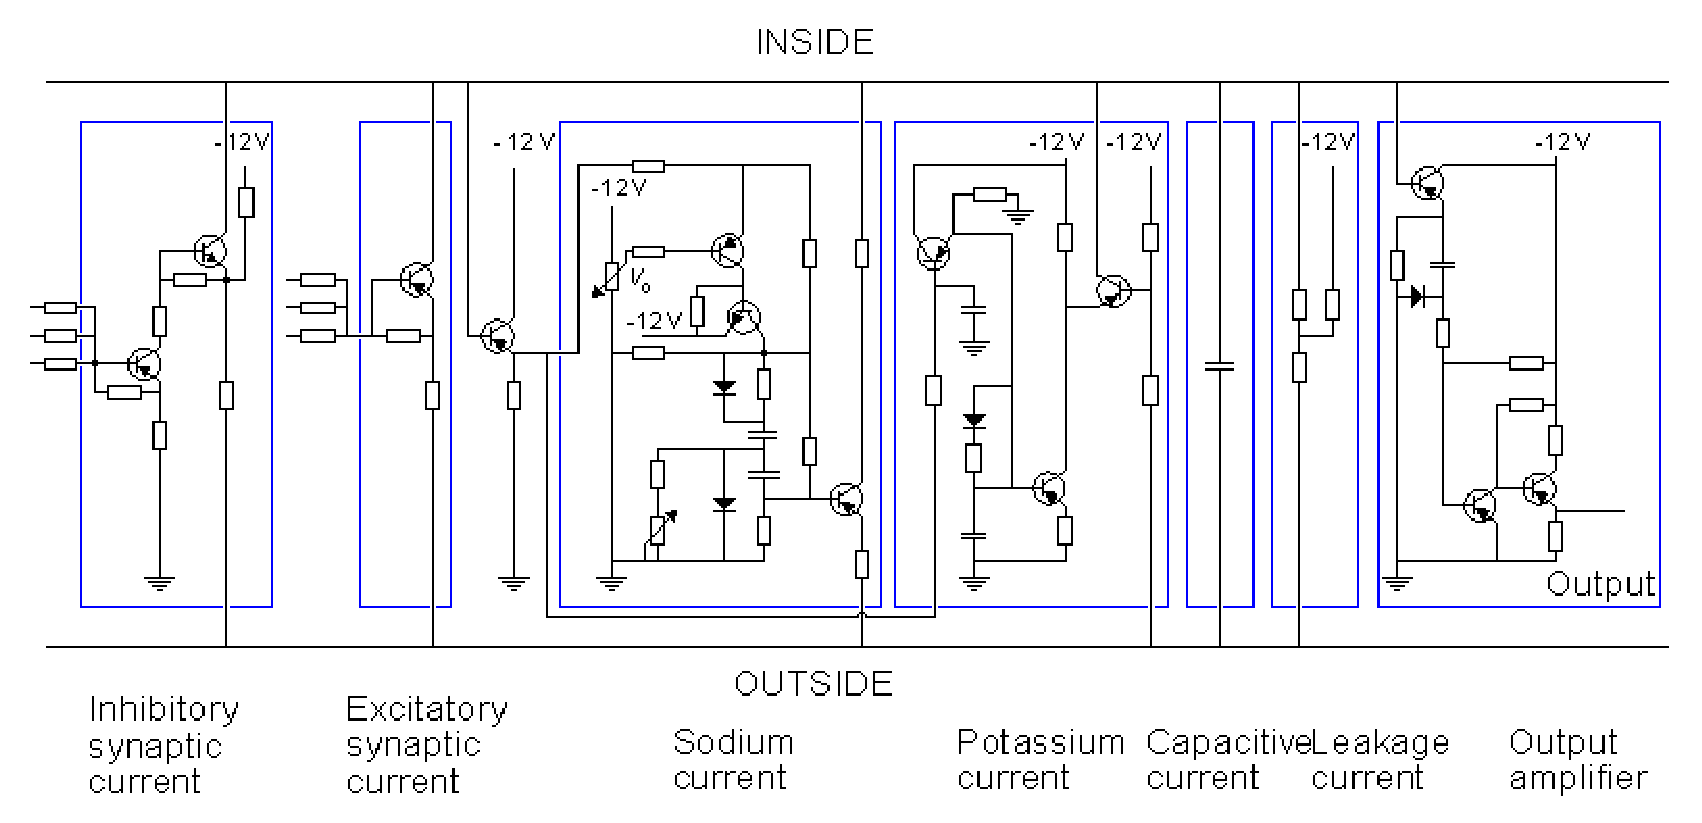
\includegraphics[width=0.8\textwidth]{figures/lewis_neuron}
	\caption{The Lewis neuron model from 1968.}
\end{figure}


The electronic realizations of the Hodgkin-Huxley model are very accurate in simulating the
function of a single neuron. However, when one is trying to simulate the function of neural 
networks, they become very complicated. 
Many scientists feel that when simulating large neural networks, the internal construction of 
its element may not be too important. It may be satisfactory simply to ensure that the elements 
produce an action pulse in response to the stimuli in a manner similar to an actual neuron. 
On this basis, Leon D. Harmon constructed a neuron model having a very simple circuit.
With this model he performed experiments in which he simulated many functions characteristic of
the neuron.
The circuit of the Harmon neuron model is given in Figure \ref{fig:harmon}.
The model is equipped with five excitatory inputs which can be adjusted. 
These include diode circuits representing various synaptic functions. 
The signal introduced at excitatory inputs charges the 0.02 $\mu F$ capacitor which, after reaching
a voltage of about 1.5 V, allows the monostable multivibrator, formed by transistors T1 and T2, 
to generate the action pulse. This impulse is amplified by transistors T3 and T4. 
The output of one neuron model may drive the inputs of perhaps 100 neighboring neuron models.
The basic model also includes an inhibitory input. A pulse introduced at this input has the effect
of decreasing the sensitivity to the excitatory inputs.. 
\begin{figure}[htb] 
	\label{fig:harmon}
	\centering
	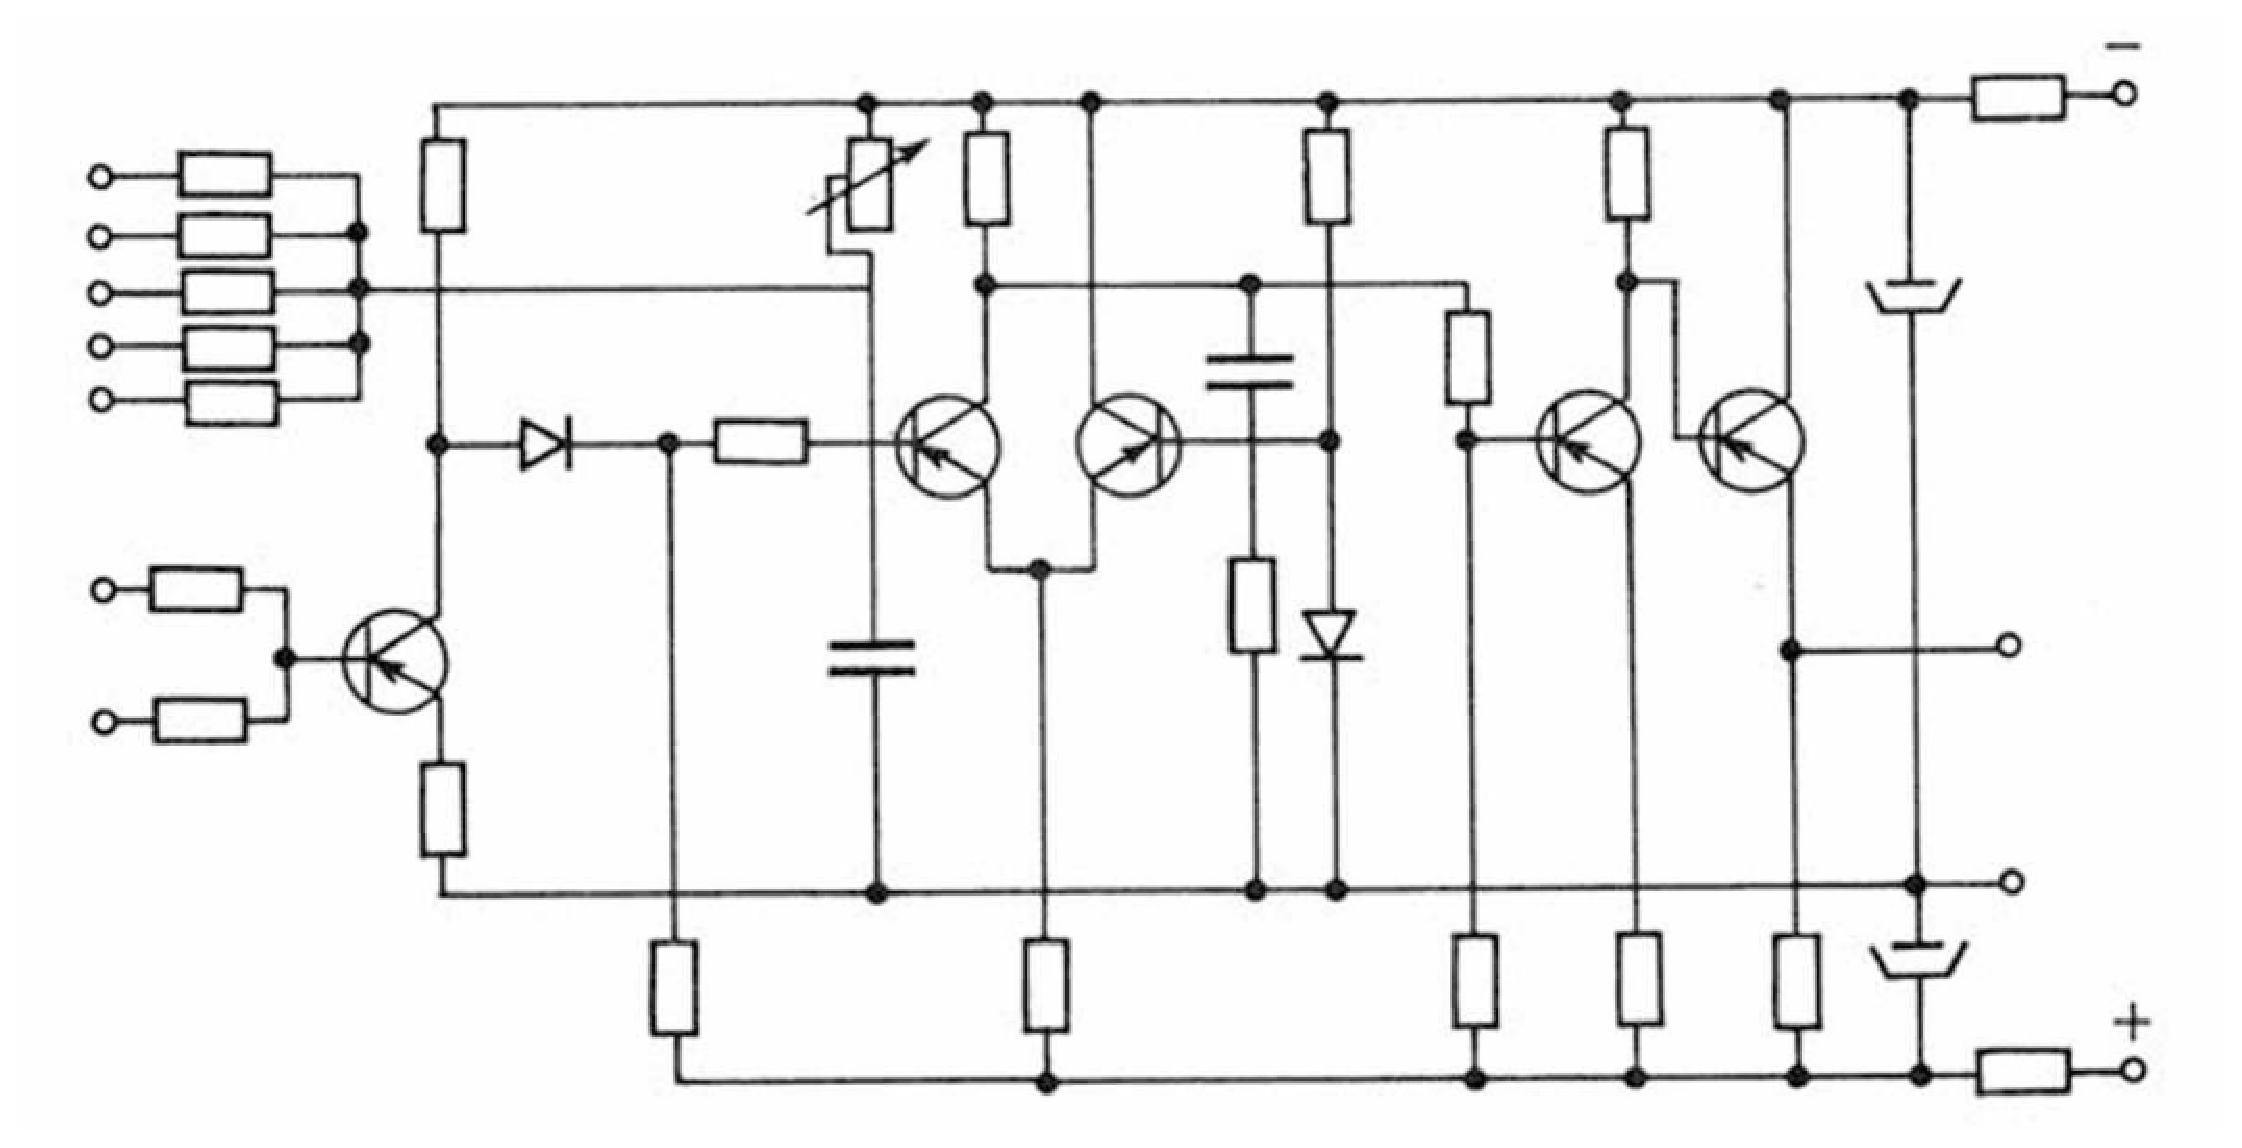
\includegraphics[width=0.8\textwidth]{figures/harmon}
	\caption{Harmon electrical model of neurall cell}
\end{figure}
%----------------------------------------------------------------------------------------------------
\subsection{Artificial representation of biological neuron}
\FloatBarrier
In 1943 Warren S. McCulloch, a neuroscientist, and Walter Pitts, a logician, 
published "A logical calculus of the ideas immanent in nervous activity" in the 
Bulletin of Mathematical Biophysics 5:115-133. In this paper McCulloch and Pitts tried to
understand how the brain could produce highly complex patterns by using many basic cells
that are connected together. 
McCulloch Pitts neuron is a highly simplified model of neural cell that models only a most
basic behavior of electrical signal transmition.
Neuron is divided into three blocks:
\begin{enumerate}
	\item aggregation where many input signals $\{x_{1}, x_{2}, \cdots, x_{n}\}$ are 
		aggregated into single signal $\hat{u}$,
	\item dampening where signal strength is reduced according to bias term and dampened 
		response $u$ is returned,
	\item activation where signal $u$ is transformed to neuron response space.
\end{enumerate}
Response of neuron modelled like that can be written as:
\begin{equation}
	\label{equ:neuron_response}
	h_{x} = f_{a}(u(\hat{u}(x))),
\end{equation}
however as in most cases weighted sum is realisation of aggregation and dampening is handled by
a simple substation neuron equation is simplified to: 
\begin{equation}
	\label{equ:neuron_response}
	h_{x} = f_{a}(u(x)).
\end{equation}
In case of McCulloch Pitts neuron both aggregation and dampening are realised by a single 
linear function akin to linear predictor:
\begin{equation}
	\label{equ:linear_neuron}
	u(x) = \Theta_{0} + \Theta_{1}x_{1} + \cdots + \Theta_{n}x_{n},
\end{equation}
which as described in chapter \ref{sec:linear_regression} can be written in a matrix notation as
\begin{equation}
	\label{equ:linear_neuron_matrix}
	u(X) = \Theta^{T}\cdot X.
\end{equation}
Almost all modern implementations of artificial neural networks use this aggregation, dampening
model and the only difference between them is in an activation function.
McCulloch Pitts neuron uses step function as an activation:
\[
	\label{equ:step_function}
	 f_{STEP}(u)=
	\begin{cases}
		1,&  u > 0, \\
		0,&  u \leq 0,
	\end{cases}
	.
\]
With this function neuron can process signals however it still lacks a very important function
of a biological neuron, ability to learn. First learning algorithm developed on base of 
McCulloch Pitts neuron was perceptron algorithm created by \textbf{TODO: BY WHO}.
With $\hat{y}$ defined as a neuron prediction and $y$ as a expected output perceptron learning
algorithm can me described as:
\begin{enumerate}
	\item if $\hat{y}=y$ then do nothing,
	\item if $\hat{y}=1$ and $y=0$ then $\Theta \leftarrow \Theta + x$
	\item if $\hat{y}=0$ and $y=1$ then $\Theta \leftarrow \Theta - x$
\end{enumerate}
Due to its ability to separate space into two subspaces perceptron can be used to model a logical
operators and as such realise logical reasoning.
Let's start with the AND operator.  Looking back at the logic table for the $A\land B$, 
we can see that we only want the neuron to output a 1 when both inputs are activated.
To do this, we want the sum of both inputs to be greater than the threshold, but each input alone
must be lower than the threshold.  Let's use a threshold of 1. 
So, now we need to choose the weights according to the constraints I've just explained - 
how about 0.6 and 0.6?  With these weights, individual activation of either input A or B will 
not exceed the threshold, while the sum of the two will be 1.2, which exceeds the threshold 
and causes the neuron to fire.
I've used a greek letter theta to denote the threshold, which is quite common practice. 
A and B are the two inputs.  You can think of them as input neurons, like photoreceptors, 
taste buds, olfactory receptors, etc.  They will each be set to 1 or 0 depending upon the truth of
their proposition.  The red neuron is our decision neuron. 
If the sum of the synapse-weighted inputs is greater than the threshold, 
this will output a 1, otherwise it will output a 0.  
So, to test it by hand, we can try setting A and B to the different values in the 
truth table and seeing if the decision neuron's output matches the $A\land B$ column:
\begin{itemize}
	\item  $A=0 \land B=0  \to   \hat{y} = 0*1  +  0*1 - 1  = -1 \to$,
	\item $A=0 \land B=1  \to  \hat(y) = 0*1  +  1*1  = 0.6$,
	\item $A=1 \land B=0  \to  \hat(y) = 1*1  +  0*1  = 0.6$,
	\item $A=1 \land B=1  \to  \hat(y) = 1*1  +  1*1  = 1.2$.
\end{itemize}

We have designed a neuron which implements a logical AND gate.  

This is easy to implement in Excel.  In fact, it's exactly the same as the neuron we 
created in What does a neuron do.  

Next up is the OR gate.  Look back at the logic table.  In this case, we want the output to 
be 1 when either or both of the inputs, A and B, are active, but 0 when both of the inputs are 0.  
This is simple enough.  If we make each synapse greater than the threshold, 
then it'll fire whenever there is any activity in either or both of A and B.
This is shown on the right.  Synaptic values of 1.1 are sufficient to surpass 
the threshold of 1 whenever their respective input is active.  
	

%====================================================================================================
\section{Artificial neural networks}

%----------------------------------------------------------------------------------------------------
\subsection{Feed forward neural networks}
\FloatBarrier

\begin{figure}[htb] 
	\label{fig:xor_gates}
	\centering
	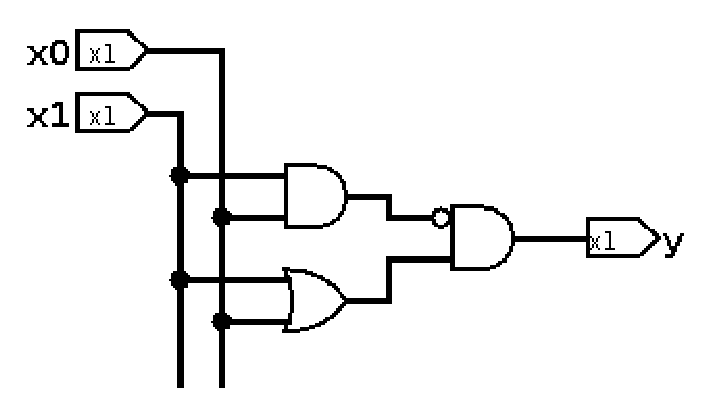
\includegraphics[width=0.6\textwidth]{figures/xor_gates}
	\caption{Implementation of XOR gate with AND, OR and NOT gates}
\end{figure}

\begin{figure}[htb] 
	\label{fig:neuro_xor}
	\centering
	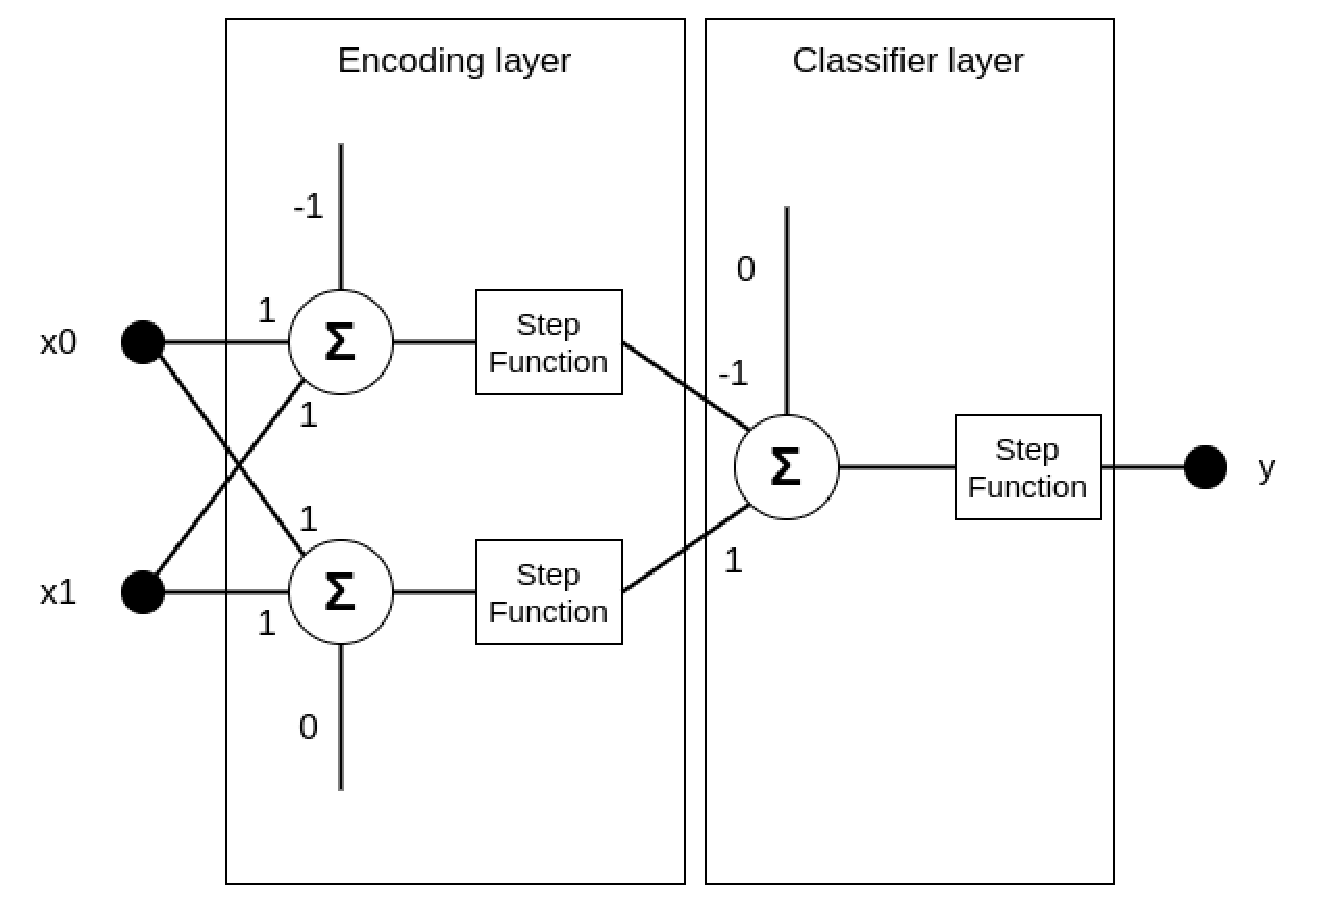
\includegraphics[width=\textwidth]{figures/neuro_xor}
	\caption{Neuron based equivalent of XOR function}
\end{figure}

%----------------------------------------------------------------------------------------------------
\subsection{Simple recurrent neural networks}
Simple solution to problem of time independence is to concatenate response of neural layer
from previous cycle to it input 
\begin{equation}
	\label{equ:sru_input}
	x'(t)=[x(t)|y(t-1)]
\end{equation}
Such solution results in signal propagating trough time and influencing responses of future cycles,
if this is only modification to feed forward model such layer is called simple recurrent
unit (SRU).
While this solution makes model time aware it have its own problems, mainly a signal vanishing
issue. Since the input signal from cycle $n$ have direct influence only on a response of this
cycle and for each subsequent cycles it is only trough feedback loop. Influence of input $n$ on
response of cycle $n+k$ grows inverse proportional to $k$.
This means that in this model only those regularities that appear over short time periods can
be detected.
Making weights on feedback bigger will not eliminate problem and instead replace it with signal
explosion that causes response to reach maximum value if a strong signal appeared on input at
least once.

%----------------------------------------------------------------------------------------------------
\subsection{Networks with long term memory}
\FloatBarrier
One of possible solutions to this issue is addition of long term memory which will regulate
forward and loop back path influence on neuron response, such solution is used in long short
term memory (LSTM) networks \cite{Hochreiter1997}.
\begin{figure}[htb] 
	\label{fig:lstm}
	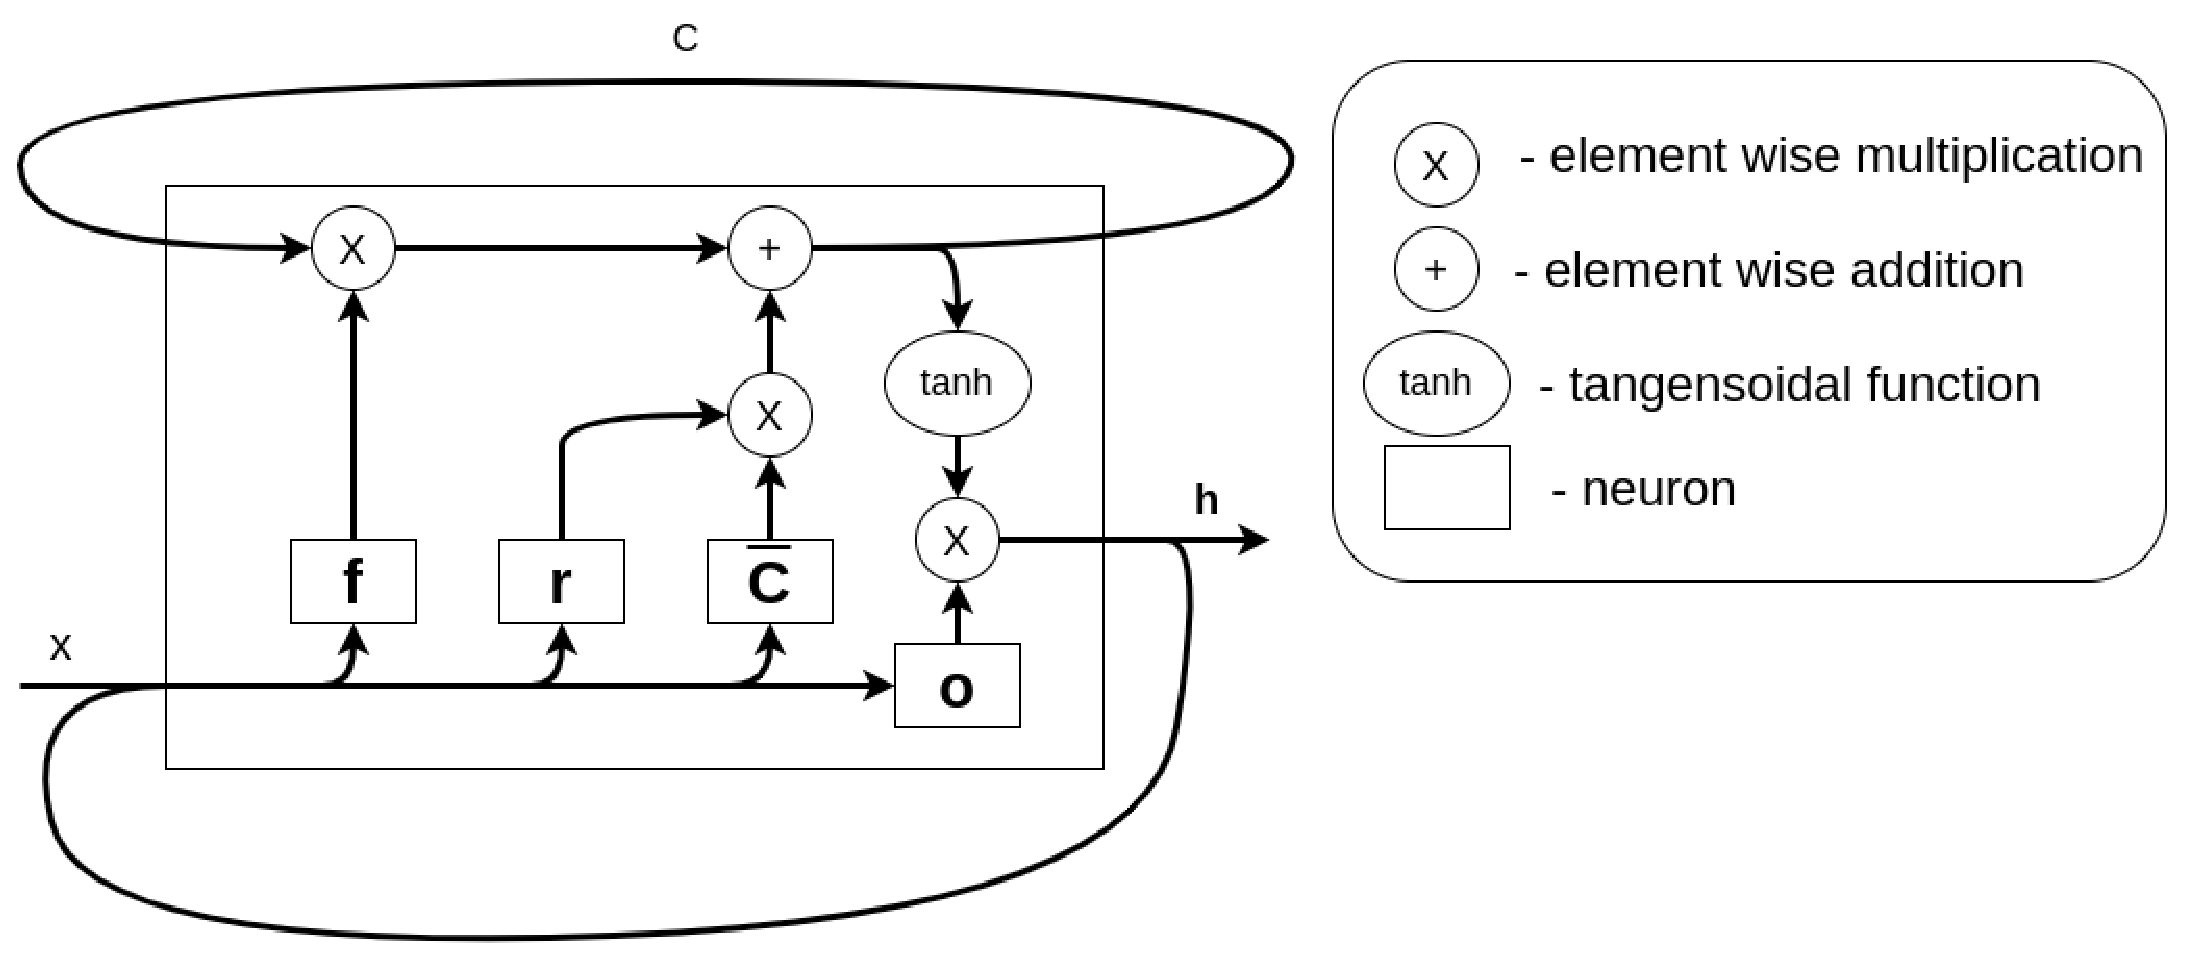
\includegraphics[width=\textwidth]{figures/lstm}
	\caption{LSTM layer}
\end{figure}
Single LSTM neuron consists of 4 basic neurons and two non neuron operations:
\begin{itemize}
\item $x'(t)=[x(t)|y(t-1)]$,
\item $o_t=\sigma (W_o\cdot x'_t+b_o)$,
\item $r_t=\sigma (W_r\cdot x'_t+b_r)$,
\item $f_t=\sigma (W_f\cdot x'_t+b_f)$,
\item $\bar{C}_t=\tanh (W_c\cdot x'_t+b_c)$,
\item $C_t=f_t\circ C_{t-1}+r_t\circ \bar{C}_t$,
\item $y_t=o_t\circ \tanh (C_t)$.
\end{itemize}
With $W$ and $b$ being weights and biases for each basic neuron, $x$ input, $y$ output and
$C$ long term memory. As it can be seen $o_t$ is a equivalent of SRU and is moderated by
long term memory before propagating as output. Temporary value of long term memory based
only on current output $\bar{C}_t$ is calculated and then with help of neurons $r$ and $f$
is transformed into its final value.
Neuron $r$ is called remembering gate and influences to what degree temporary long term
memory from given cycle effects its final value while $f$ is forgetting gate and
decides influence of long term memory from last cycle on current one.
Thanks to such implementation model can learn to detect long term regularities as well
as short term ones.
Gated recurrent units (GRUs) are a gating mechanism in recurrent neural networks,
introduced in 2014 by Kyunghyun Cho et al.
The GRU is like a long short-term memory (LSTM) with a forget gate, but has fewer parameters 
than LSTM, as it lacks an output gate. GRU's performance on certain tasks of polyphonic music
modeling, speech signal modeling and natural language processing was found to be similar 
to that of LSTM. GRUs have been shown to exhibit better performance on certain smaller and less
frequent datasets.
\begin{figure}[htb] 
	\label{fig:gru}
	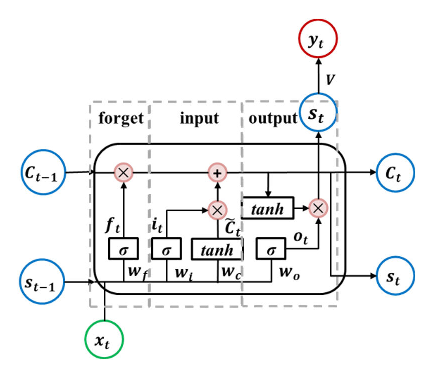
\includegraphics[width=0.7\textwidth]{figures/gru}
	\caption{GRU layer}
\end{figure}
The minimal gated unit is similar to the fully gated unit, except the update and reset gate vector
is merged into a forget gate. This also implies that the equation for the output vector 
must be changed.

%----------------------------------------------------------------------------------------------------
\subsection{Backpropagation Through Time}
\FloatBarrier
Backpropagation Through Time (BPTT) is the algorithm that is used to update the weights in the 
recurrent neural network. 
One of the common examples of a recurrent neural network is LSTM. 
Backpropagation is an essential skill that you should know if you want to effectively frame 
sequence prediction problems for the recurrent neural network. You should also be aware of the
effects of the Backpropagation Through time on the stability, the speed of the system while 
training the system.
The ultimate goal of the Backpropagation algorithm is to minimize the error of the network outputs.

The Backpropagation Through Time is the application of Backpropagation training algorithm which 
is applied to the sequence data like the time series. It is applied to the 
recurrent neural network. 
The recurrent neural network is shown one input each timestep and predicts the corresponding
output. So, we can say that BTPP works by unrolling all input timesteps.
Each timestep has one input time step, one output time step and one copy of the network.
Then the errors are calculated and accumulated for each timestep.
The network is then rolled back to update the weights.
But one of the disadvantages of BPTT is when the number of time steps increases the computation
also increases. This will make the overall model noisy. The high cost of single parameter updates
makes the BPTT impossible to use for a large number of iterations.
This is where Truncated Backpropagation comes save the day for us. 
Truncated Backpropagation (TBPTT) is nothing but a slightly modified version of BPTT algorithm 
for the recurrent neural network. In this, the sequence is processed one timestep at a time and
periodically the BPTT update is performed for a fixed number of time steps.

The basic Truncated Backpropagation algorithm is
\begin{enumerate}
    \item First, give the sequence of, say K1 time steps of input and output pairs to the network.
    \item Then calculate and accumulate the errors across say, k2 time steps 
		by unrolling the network
    \item Finally, update the weights by rolling up the network
\end{enumerate}
As you can clearly see that you need two parameters namely k1 and k2 for implementing TBPTT. 
K1 is the number of forwarding pass timesteps between updates.
This influences how fast or slow will be the training and the frequency of the weight updates. 
On the other hand, k2 is the number of timesteps which apply to BPTT. 
It should be large enough to capture the temporal structure in the problem 
for the network to learn. 

%====================================================================================================
\section{Overfitting}
\FloatBarrier
Overfitting is a concept in data science, which occurs when a statistical model fits exactly
against its training data. 
When this happens, the algorithm unfortunately cannot perform accurately against unseen data,
defeating its purpose.
Generalization of a model to new data is ultimately what allows us to use machine learning
algorithms every day to make predictions and classify data.
When machine learning algorithms are constructed, they leverage a sample dataset 
to train the model. 
However, when the model trains for too long on sample data or when the model is too complex, 
it can start to learn the “noise,” or irrelevant information, within the dataset. 
When the model memorizes the noise and fits too closely to the training set, 
the model becomes “overfitted,” and it is unable to generalize well to new data.
If a model cannot generalize well to new data, then it will not be able to perform the
classification or prediction tasks that it was intended for.

Low error rates and a high variance are good indicators of overfitting.
In order to prevent this type of behavior, part of the training dataset is typically set aside 
as the “test set” to check for overfitting. 
If the training data has a low error rate and the test data has a high error rate, 
it signals overfitting.

%----------------------------------------------------------------------------------------------------
\subsection{Early stoppingi}
\FloatBarrier
Regularization by early stopping can be done either by dividing the dataset into training and test 
sets and then using cross-validation on the training set or by dividing the dataset into training, 
validation and test sets, in which case cross-validation is not required.
Here, the second case is analyzed. In early stopping, the algorithm is trained using the
training set and the point at which to stop training is determined from the validation set. 
Training error and validation error are analysed. The training error steadily decreases while 
validation error decreases until a point, after which it increases. 
This is because, during training, the learning model starts to overfit to the training data. 
This causes the training error to decrease while the validation error increases.
So a model with better validation set error can be obtained if the parameters that give the least
validation set error are used.
Each time the error on the validation set decreases, a copy of the model parameters is stored.
When the training algorithm terminates, these parameters which give the least validation set
error are finally returned and not the last modified parameters. 
\begin{figure}[htb] 
	\label{fig:early_stop}
	\centering
	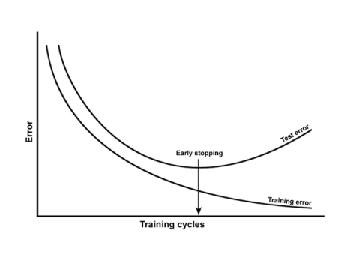
\includegraphics[width=0.6\textwidth]{figures/early_stop}
	\caption{Neuron based equivalent of XOR function}
\end{figure}

In Regularization by Early Stopping, we stop training the model when the performance of the 
model on the validation set is getting worse-increasing loss or decreasing accuracy or poorer 
values of the scoring metric. By plotting the error on the training dataset and the validation 
dataset together, both the errors decrease with a number of iterations until the point where 
the model starts to overfit.
After this point, the training error still decreases but the validation error increases. 
So, even if training is continued after this point, early stopping essentially returns the set of
parameters which were used at this point and so is equivalent to stopping training at that point.
So, the final parameters returned will enable the model to have low variance and 
better generalization. 
The model at the time the training is stopped will have a better generalization performance than
the model with the least training error. 
Early stopping can be thought of as implicit regularization, contrary to regularization via 
weight decay. 
This method is also efficient since it requires less amount of training data,
which is not always available. Due to this fact, early stopping requires lesser time for training 
compared to other regularization methods. 
Repeating the early stopping process many times may result in the model overfitting the
validation dataset, just as similar as overfitting occurs in the case of training data.

The number of iterations taken to train the model can be considered as a hyperparameter.
Then the model has to find an optimum value for this hyperparameter(by hyperparameter 
tuning)for the best performance of the learning model.


%----------------------------------------------------------------------------------------------------
\subsection{$\ell$ regularization}
\FloatBarrier
A regression model that uses L1 regularization technique is called Lasso Regression and model i
which uses L2 is called Ridge Regression.
The key difference between these two is the penalty term.

Ridge regression adds ``squared magnitude'' of coefficient as penalty term to the loss function.
Here the highlighted part represents L2 regularization element.
\begin{equation}
	\label{equ:ridge_regression}
	\sum_{i=1}^{n}(y_{i}-\sum_{j=1}^{p}x_{ij}\beta_{j})^{2} + \lambda \sum_{j=1}^{p}\beta_{j}^{2},
\end{equation}
Here, if lambda is zero then you can imagine we get back OLS.
However, if lambda is very large then it will add too much weight and it will lead to
under-fitting. Having said that it’s important how lambda is chosen.
This technique works very well to avoid over-fitting issue.

Lasso Regression (Least Absolute Shrinkage and Selection Operator) adds
``absolute value of magnitude'' of coefficient as penalty term to the loss function.
\begin{equation}
	\label{equ:lasso_regresson}
	\sum_{i=1}^{n}(Y_{i}-\sum_{j=1}^{p}X_{ij}\beta_{j})^{2} + \lambda \sum_{j=1}^{p}
	\vert \beta_{j} \vert,
\end{equation}
Again, if lambda is zero then we will get back OLS whereas very large value will make coefficients 
zero hence it will under-fit.
The key difference between these techniques is that Lasso shrinks the less important feature’s 
coefficient to zero thus, removing some feature altogether. 
So, this works well for feature selection in case we have a huge number of features.

%----------------------------------------------------------------------------------------------------
\subsection{Dropout}
\FloatBarrier
Deep neural networks contain multiple non-linear hidden layers and this makes them very
expressive models that can learn very complicated relationships between their inputs and
outputs. With limited training data, however, many of these complicated relationships
will be the result of sampling noise, so they will exist in the training set but not in real
test data even if it is drawn from the same distribution. This leads to overfitting and many
methods have been developed for reducing it. These include stopping the training as soon as
performance on a validation set starts to get worse, introducing weight penalties of various
kinds such as L1 and L2 regularization and soft weight sharing (Nowlan and Hinton, 1992).

With unlimited computation, the best way to “regularize” a fixed-sized model is to
average the predictions of all possible settings of the parameters, weighting each setting by
its posterior probability given the training data. This can sometimes be approximated quite
well for simple or small models (Xiong et al., 2011; Salakhutdinov and Mnih, 2008), but we
would like to approach the performance of the Bayesian gold standard using considerably
less computation. We propose to do this by approximating an equally weighted geometric
mean of the predictions of an exponential number of learned models that share parameters.
Model combination nearly always improves the performance of machine learning meth-
ods. With large neural networks, however, the obvious idea of averaging the outputs of
many separately trained nets is prohibitively expensive. Combining several models is most
helpful when the individual models are different from each other and in order to make
neural net models different, they should either have different architectures or be trained
on different data. Training many different architectures is hard because finding optimal
hyperparameters for each architecture is a daunting task and training each large network
requires a lot of computation. Moreover, large networks normally require large amounts of
training data and there may not be enough data available to train different networks on
different subsets of the data. Even if one was able to train many different large networks,
using them all at test time is infeasible in applications where it is important to respond
quickly.
Dropout is a technique that addresses both these issues. It prevents overfitting and
provides a way of approximately combining exponentially many different neural network
architectures efficiently. The term “dropout” refers to dropping out units (hidden and
visible) in a neural network. By dropping a unit out, we mean temporarily removing it from
the network, along with all its incoming and outgoing connections, as shown in Figure 1.
The choice of which units to drop is random. In the simplest case, each unit is retained with
a fixed probability p independent of other units, where p can be chosen using a validation
set or can simply be set at 0.5, which seems to be close to optimal for a wide range of
networks and tasks. For the input units, however, the optimal probability of retention is
usually closer to 1 than to 0.5.
\begin{figure}[htb] 
	\label{fig:dropout}
	\centering
	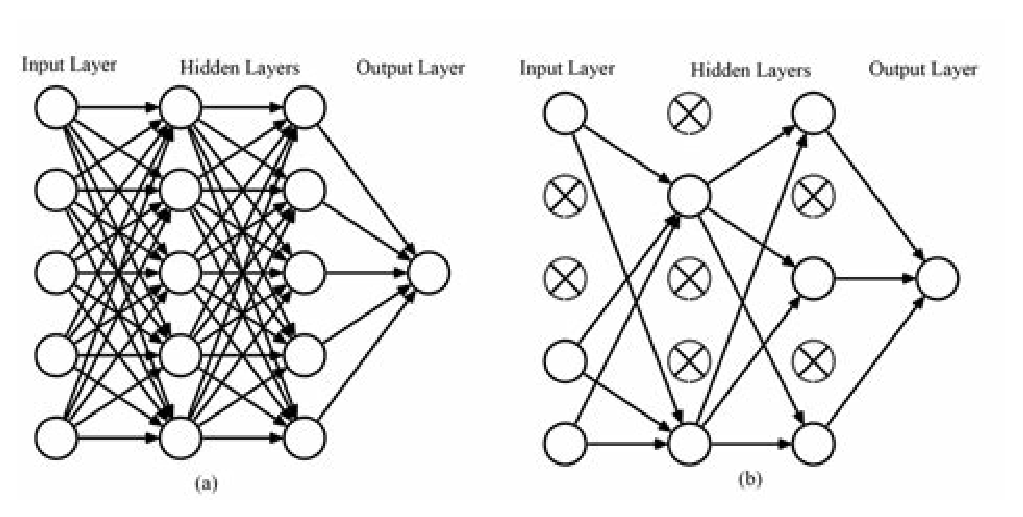
\includegraphics[width=\textwidth]{figures/dropout}
	\caption{Dropout Neural Net Model. Left: A standard neural net with 2 hidden layers.
	Right: An example of a thinned net produced by applying dropout to the network on the left.
	Crossed units have been dropped}
\end{figure}

Applying dropout to a neural network amounts to sampling a “thinned” network from
it. The thinned network consists of all the units that survived dropout (Figure 1b). A
neural net with n units, can be seen as a collection of 2 n possible thinned neural networks.
These networks all share weights so that the total number of parameters is still O(n 2 ), or
less. For each presentation of each training case, a new thinned network is sampled and
trained. So training a neural network with dropout can be seen as training a collection of 2 n
thinned networks with extensive weight sharing, where each thinned network gets trained
very rarely, if at all.
At test time, it is not feasible to explicitly average the predictions from exponentially
many thinned models. However, a very simple approximate averaging method works well in
practice. The idea is to use a single neural net at test time without dropout. The weights
of this network are scaled-down versions of the trained weights. If a unit is retained with
probability p during training, the outgoing weights of that unit are multiplied by p at test
time as shown in Figure 2. This ensures that for any hidden unit the expected output (under
the distribution used to drop units at training time) is the same as the actual output at
test time. By doing this scaling, 2 n networks with shared weights can be combined into
a single neural network to be used at test time. We found that training a network with
dropout and using this approximate averaging method at test time leads to significantly
lower generalization error on a wide variety of classification problems compared to training
with other regularization methods.
The idea of dropout is not limited to feed-forward neural nets. It can be more generally
applied to graphical models such as Boltzmann Machines. In this paper, we introduce
the dropout Restricted Boltzmann Machine model and compare it to standard Restricted
Boltzmann Machines (RBM). Our experiments show that dropout RBMs are better than
standard RBMs in certain respects.
This paper is structured as follows. Section 2 describes the motivation for this idea.
Section 3 describes relevant previous work. Section 4 formally describes the dropout model.
Section 5 gives an algorithm for training dropout networks. In Section 6, we present our
experimental results where we apply dropout to problems in different domains and compare
it with other forms of regularization and model combination. Section 7 analyzes the effect of
dropout on different properties of a neural network and describes how dropout interacts with
the network’s hyperparameters. Section 8 describes the Dropout RBM model. In Section 9
we explore the idea of marginalizing dropout. In Appendix A we present a practical guide
for training dropout nets. This includes a detailed analysis of the practic.
